\clearpage

\section{\label{systematic}Systematic Uncertainties}

The approach for the $D^0$ spectrum systematic uncertainties are well studied. Several sources can be contributed to the uncertainties. The first one is coming from the raw yield extraction. We varied the signals extraction methods instead of use binning counting methods we tried using fitting method to estimate the uncertainties for yield extraction. The second one is from the TPC embedding uncertainties, this one is well studied before in STAR collaboration and we quota 3\% for single track, 2\% for the secondary track contribution. The next one is from the fast-simulation part, as discussed in the previous section, there are $\sim$5\% difference between the pure Hijing and fast-simulation relay on Hijing when we validating the packages. We quote this 5\% contribution as one of the systematic sources.
%Another source would be the vertex resolution contribution as we discussed before, since the most central collisions does not suffer the vertex contribution while the impact on the most peripheral collisions could be visible. We quote a separate systematic errors for difference centralities, 10\% for the most peripheral (40-80\%) collision, 5\% for the mid-central collisions (10-40\%) and 0 for the most central (0-10\%) collisions. 
%The next one source coming from the bin shift correction, there are several functions can be used for the bin correction such as the levy function and fonll function, the difference between these two methods are quoted as one of the systematic source. 
The next source is by varying the topological cuts and daughter $p_t$ cuts. The standard TMVA cuts, the 50\% efficiency and 150\% efficiency cuts are calculated, and also the daughter $p_T$ cuts are checked for 300 MeV and 500 MeV beside of the default value 600 MeV. The difference between the corrected yield are quoted as the systematic source. Also there is a source coming from the double counting as we discussed in the previous section.

Fig.~\ref{sysErr_0_10} to Fig.~\ref{sysErr_0_80} shows the $D^0$ spectrum different sources contribution in various centralities. As we see, the systematic uncertainties is quite small in the most of the $p_T$ range except some of the $p_T$ ranges due to the limited statistics and large contribution from yield extraction.

\begin{figure}[htbp]
\begin{minipage}[htbp]{0.47\linewidth}
\centering
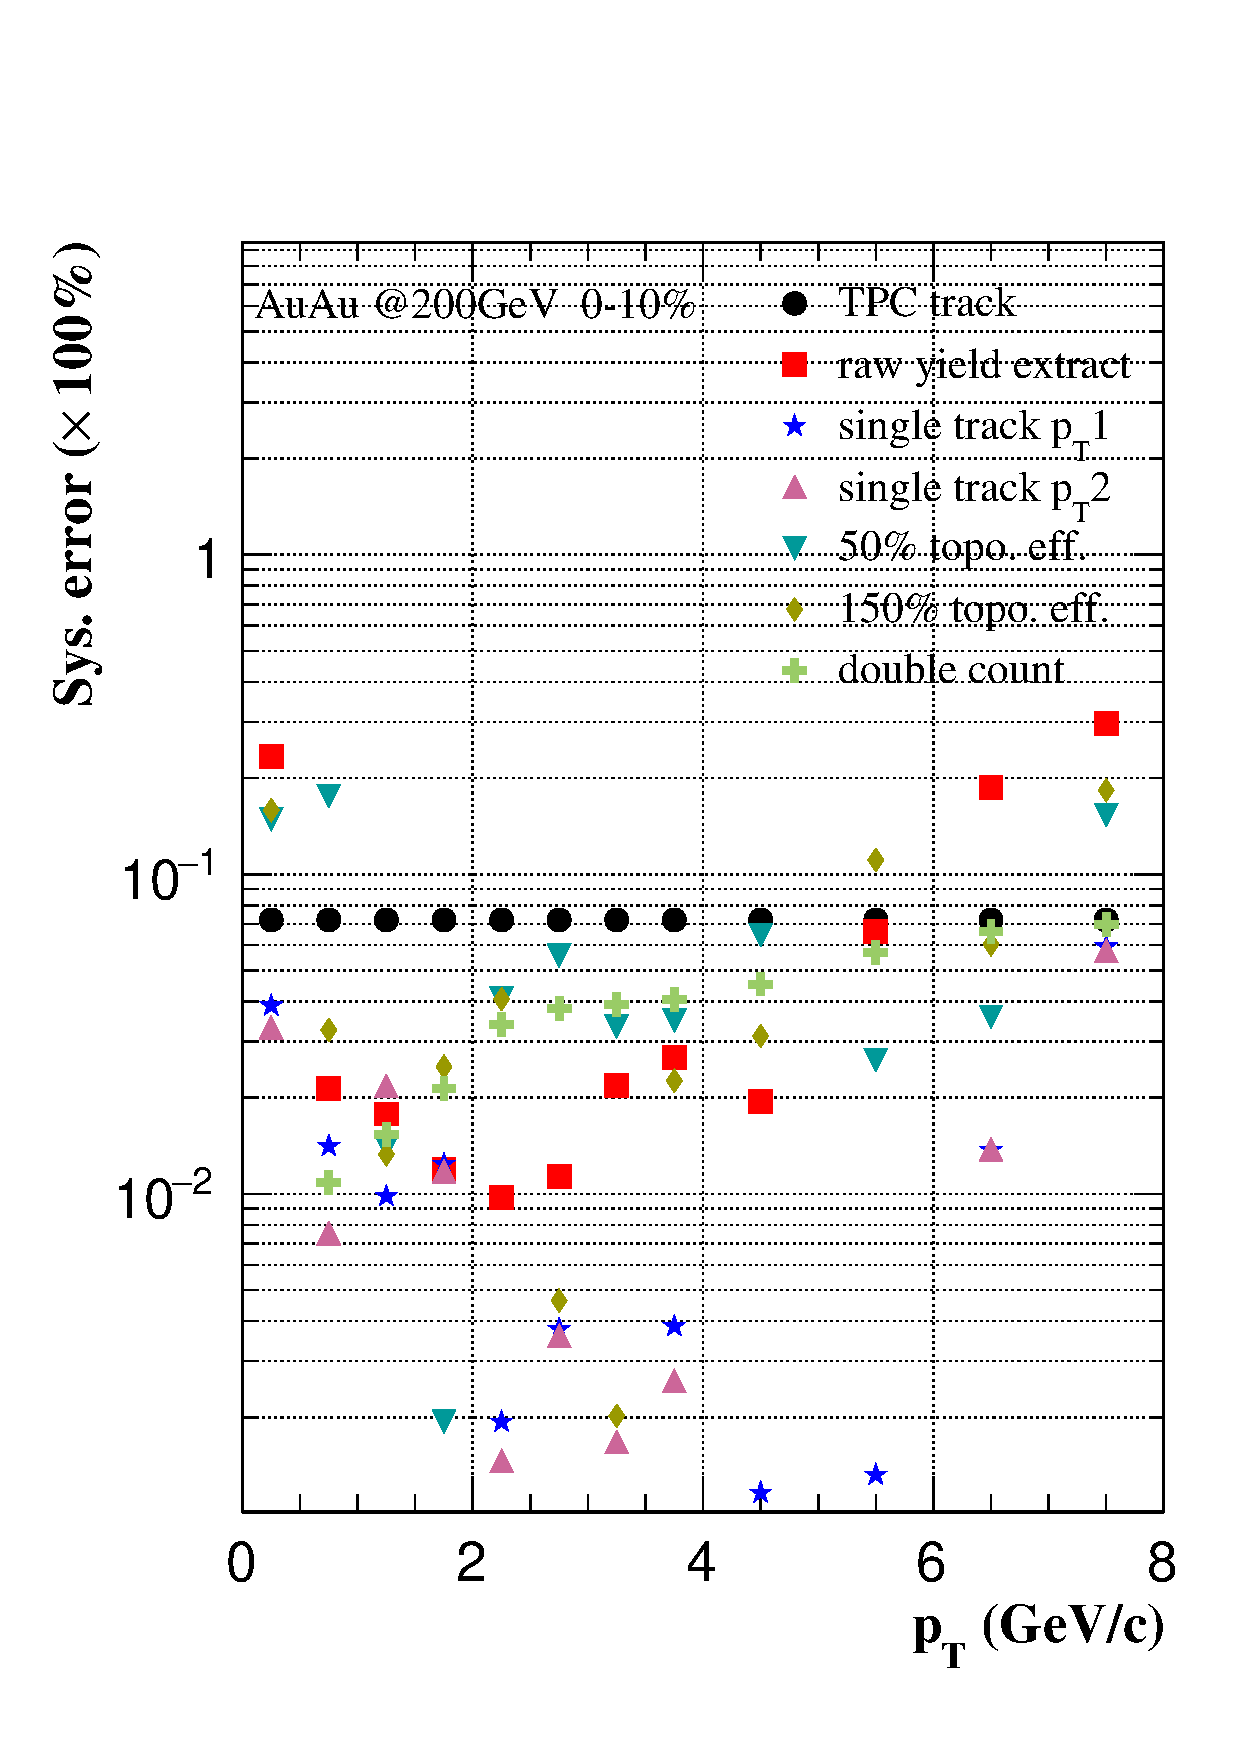
\includegraphics[width=1.0\textwidth,angle=0]{figure/Run14_D0HFT/sysErr_0_10.pdf}
\caption{ Systematic uncertainties from different sources for 0-10\%. \label{sysErr_0_10}}
\end{minipage}
\hfill
\begin{minipage}[htbp]{0.47\linewidth}
\centering
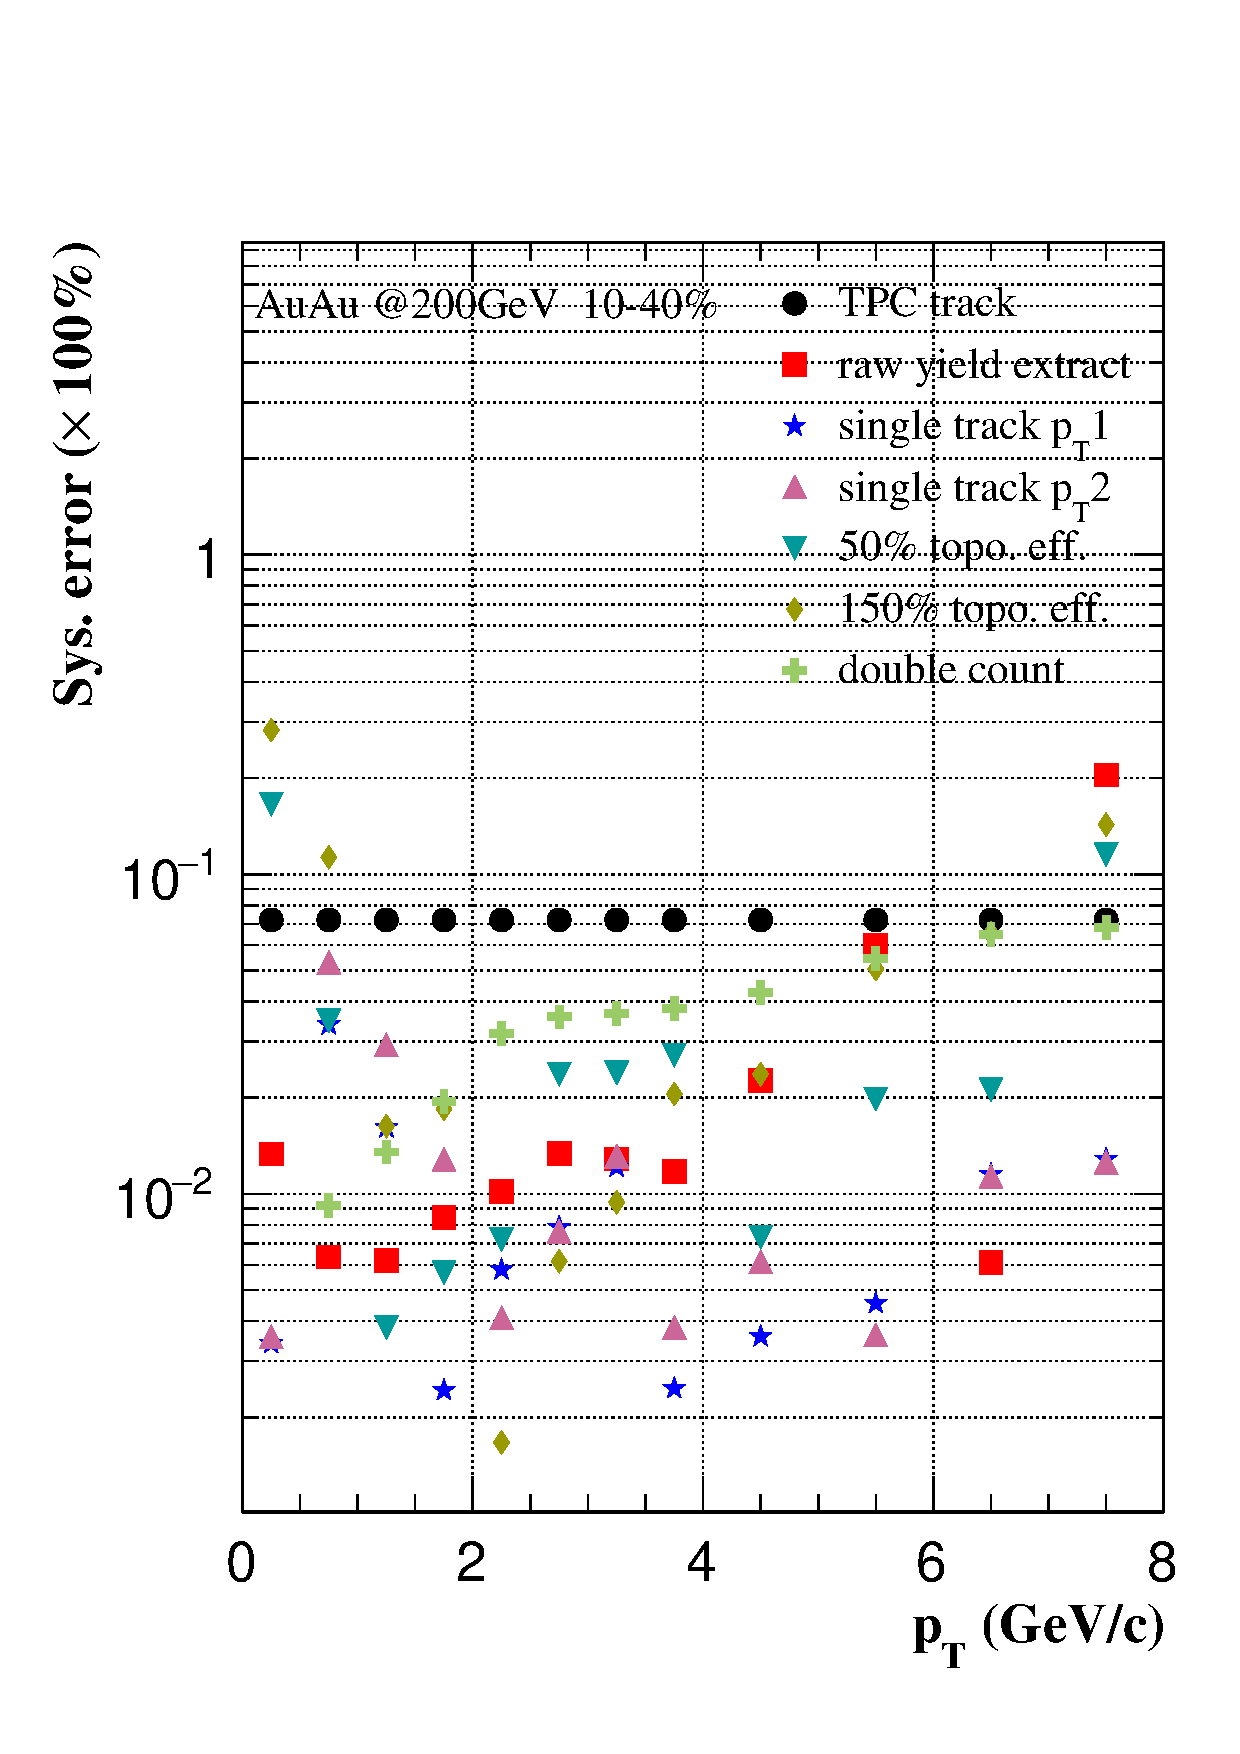
\includegraphics[width=1.0\textwidth,angle=0]{figure/Run14_D0HFT/sysErr_10_40.pdf} 
\caption{ Systematic uncertainties from different sources for 10-40\%. \label{sysErr_10_40}}
\end{minipage}
\end{figure}

\begin{figure}[htbp]
\begin{minipage}[htbp]{0.47\linewidth}
\centering
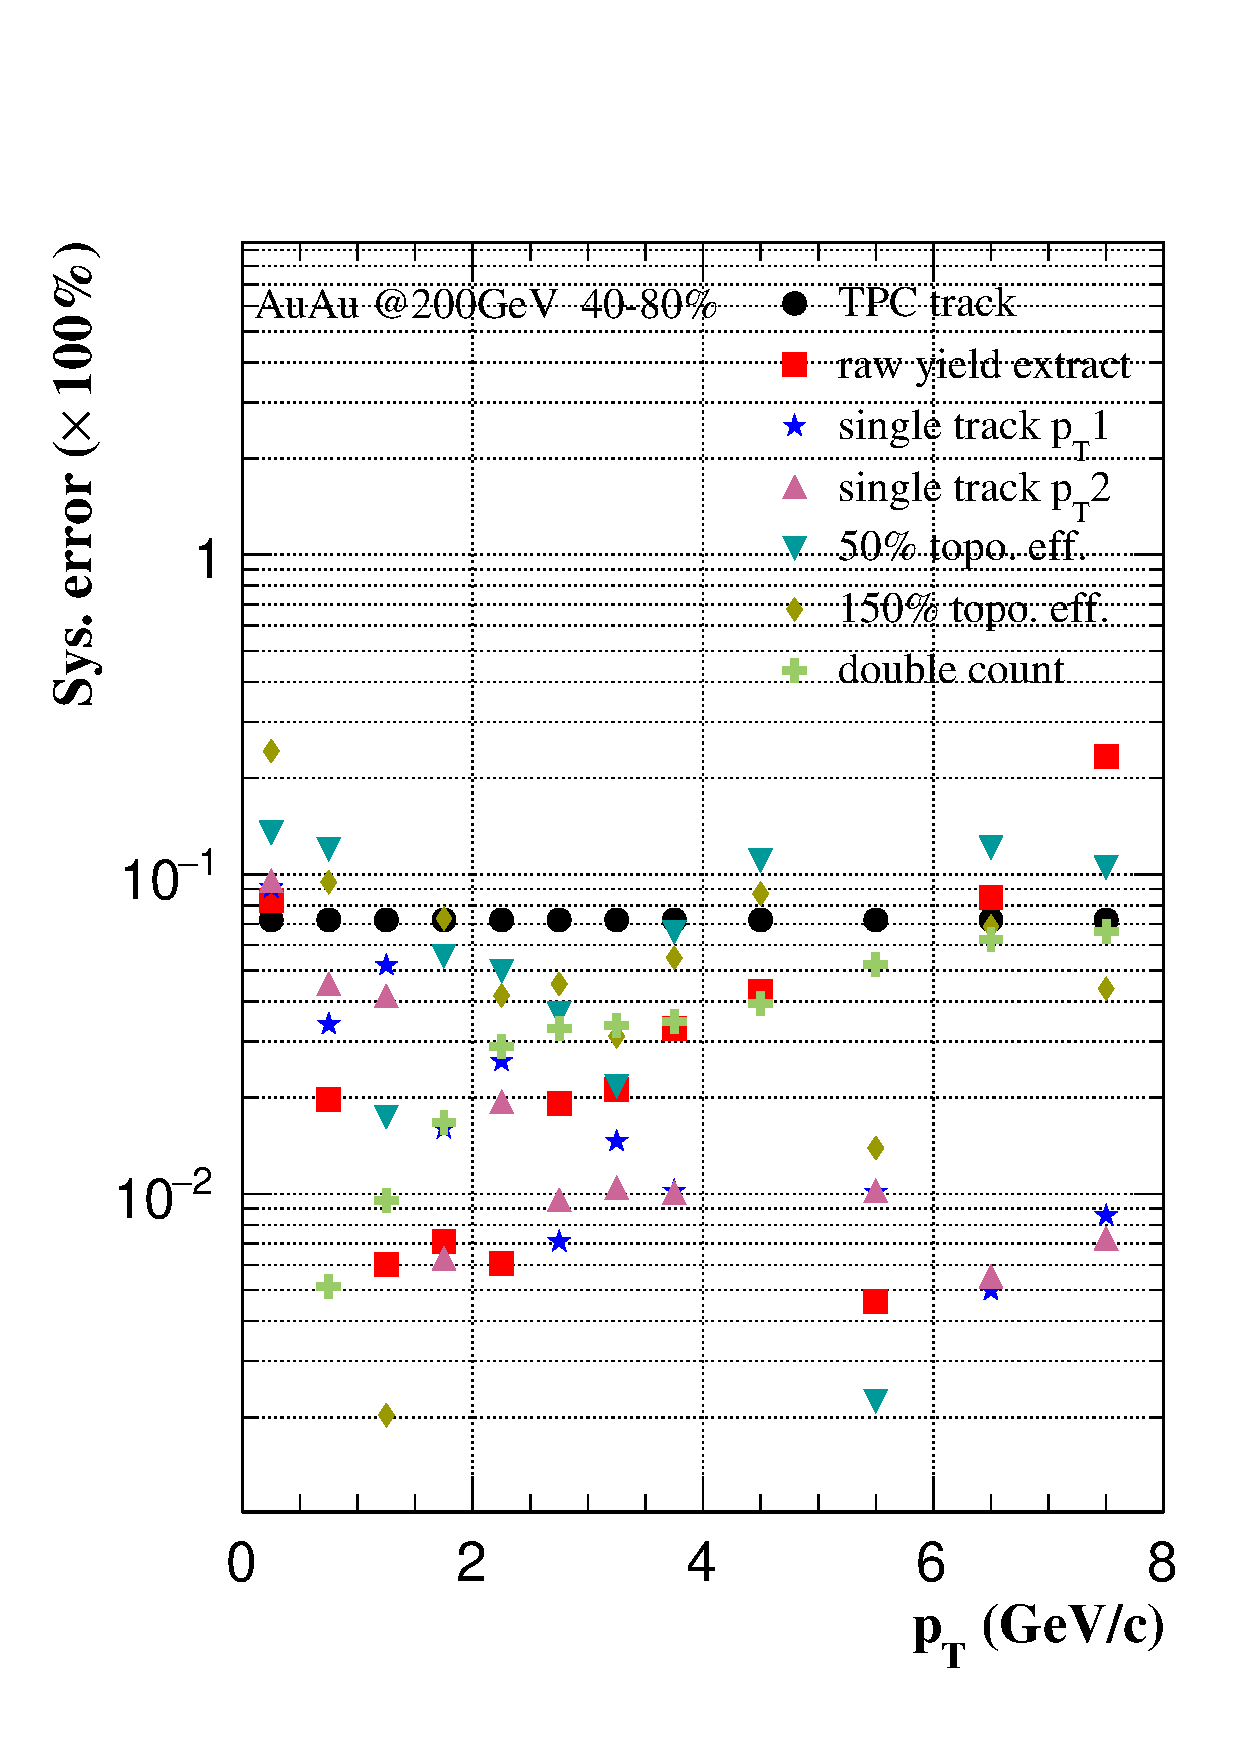
\includegraphics[width=1.0\textwidth,angle=0]{figure/Run14_D0HFT/sysErr_40_80.pdf}
\caption{ Systematic uncertainties from different sources for 40-80\%. \label{sysErr_40_80}}
\end{minipage}
\hfill
\begin{minipage}[htbp]{0.47\linewidth}
\centering
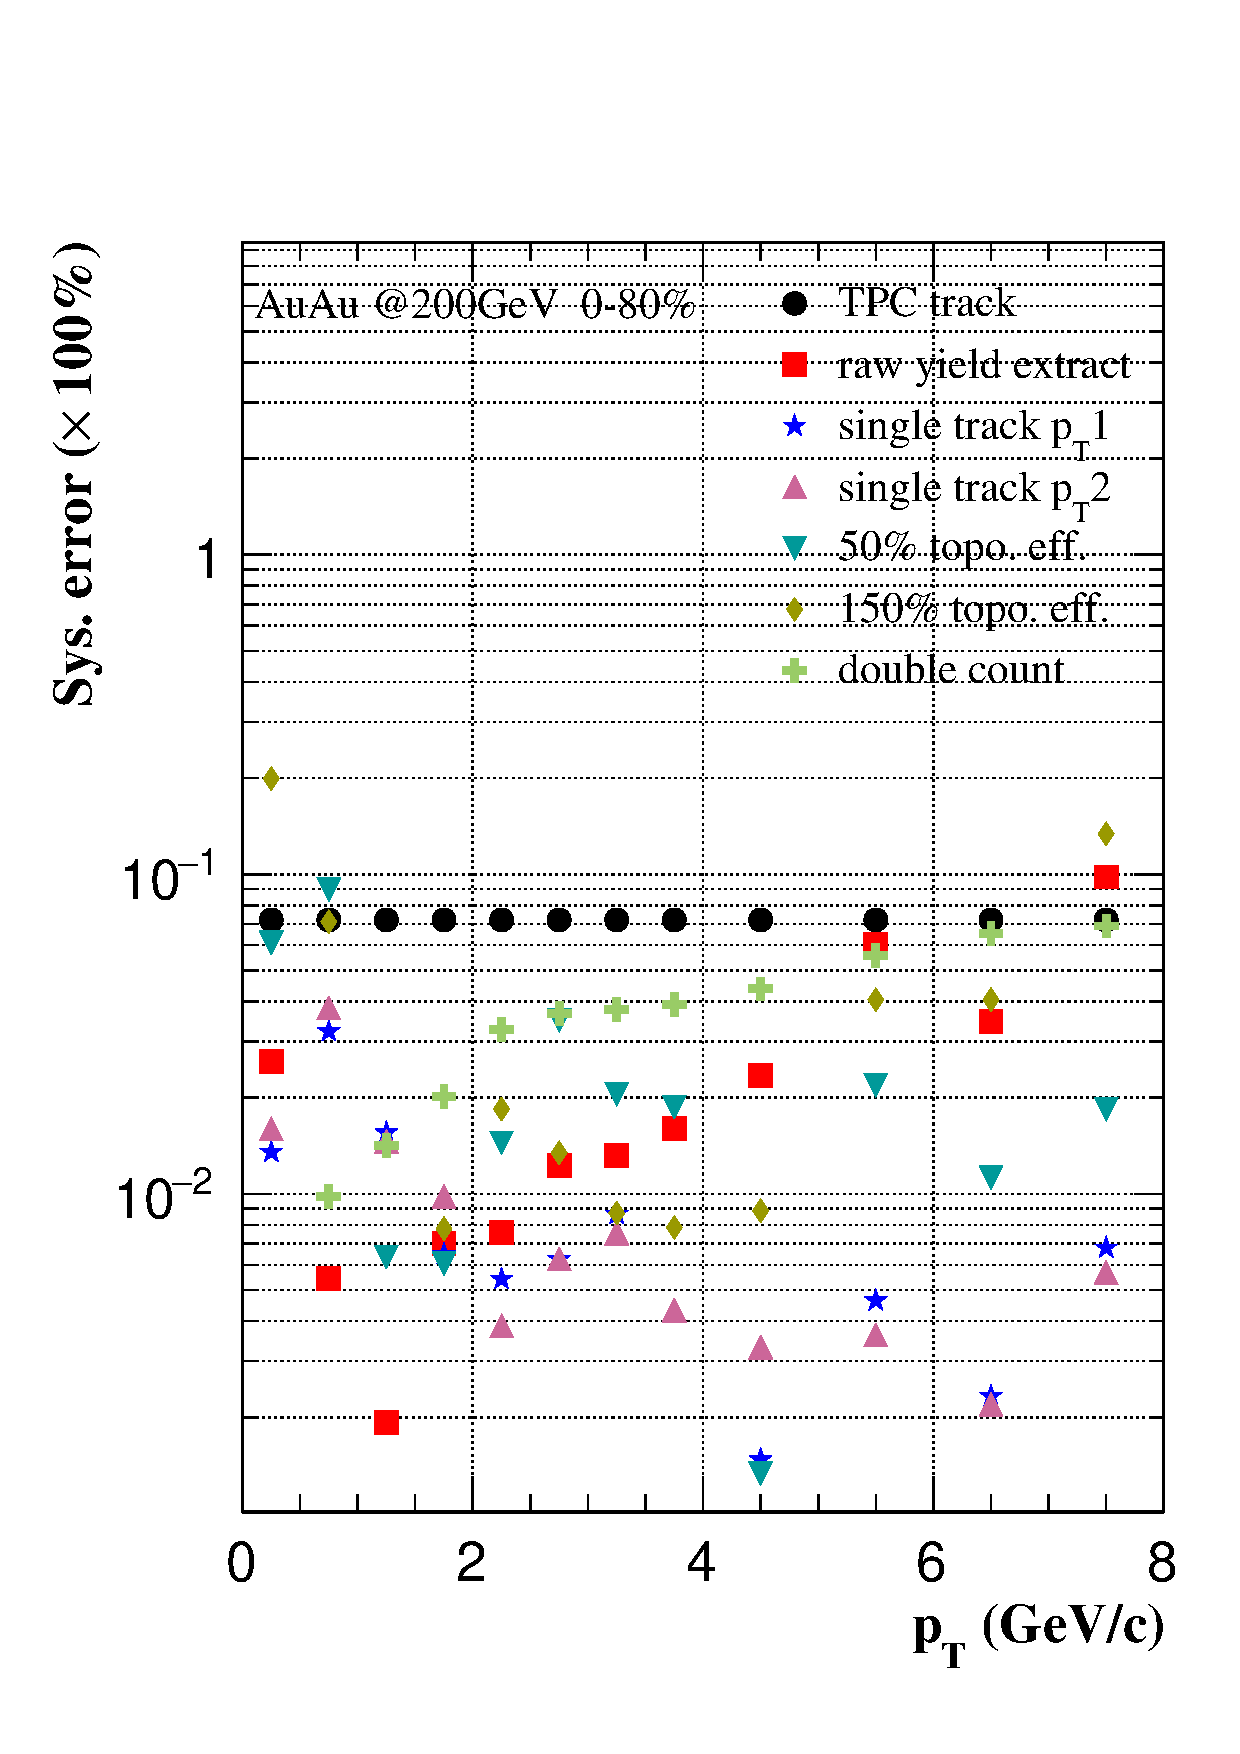
\includegraphics[width=1.0\textwidth,angle=0]{figure/Run14_D0HFT/sysErr_0_80.pdf} 
\caption{ Systematic uncertainties from different sources for 0-80\%. \label{sysErr_0_80}}
\end{minipage}
\end{figure}


% For the $R_{AA}$ results shown later, they share the most of the systematic uncertainties with the spectrum, but for the TPC part, the TPC contribution from Au+Au and p+p collisions can be canceled out. The black bracket only represented the uncertainties from Au+Au.

% \begin{table}[htp]
% \centering
% \caption{Systematic uncertainties from different sources}
% \label{syserr}
% 	\begin{center}
% 	\begin{tabular}{l|l|l|l|l|l|l|l}
%   \Xhline{1.6pt}
%   $p_T$ range&Yield extra&Embedding&fast-simu&Topo Scan&bin shift&daughter $p_T$&total\\ \hline
%   0.0 -  0.5  &   0.28575        &  0.06     &  0.05           & 0.150186  &  0.206038   &  0.0961785  &   0.402506  \\ \hline
% 	0.5 - 1.0   &   0.276043       &  0.06     &  0.05           & 0.124592  &  0.0641394  &  0.104796   &   0.336034  \\ \hline
% 	1.0 - 1.5   &   0.0332581      &  0.06     &  0.05           & 0.08445   &  0.0416632  &  0.0354619  &   0.131648  \\ \hline
% 	1.5 - 2.0   &   0.0284874      &  0.06     &  0.05           & 0.0430791 &  0.0179911  &  0.013235   &   0.096261  \\ \hline
% 	2.0 - 2.5   &   0.0152306      &  0.06     &  0.05           & 0.0597399 &  0.00416767 &  0.00651388 &   0.0998029 \\ \hline
%   2.5 - 3.0   &   0.0173818      &  0.06     &  0.05           & 0.0762663 &  0.00261387 &  0.00930911 &   0.11096   \\ \hline
%   3.0 - 3.5   &   0.0164046      &  0.06     &  0.05           & 0.0368647 &  0.00551249 &  0.0177607  &   0.0898551 \\ \hline
%   3.5 - 4.0   &   0.0301197      &  0.06     &  0.05           & 0.0712203 &  0.00646695 &  0.0237711  &   0.112634  \\ \hline
%   4.0 - 5.0   &   0.0736611      &  0.06     &  0.05           & 0.0615253 &  0.0312138  &  0.0214862  & 0.129411      \\ \hline
%   5.0 - 6.0   &   0.0751424      &  0.06     &  0.05           & 0.11637   &  0.0261331  &  0.0226671  & 0.162742      \\ \hline
%   6.0 - 7.0   &   0.0944053      &  0.06     &  0.05           & 0.0465479 &  0.0210969  &  0.00687676 & 0.132934      \\ \hline
%   7.0 - 8.0   &   0.0730125      &  0.06     &  0.05           & 0.409901  &  0.0169993  &  0.00289802 & 0.423966      \\ \hline
%   8.0 - 10.0  &   0.0984801      &  0.06     &  0.05           & 0.696775  & 0.048144    &  0.061042   &  0.712276    \\ \hline
%   \Xhline{1.6pt}
% 	\end{tabular}
% 	\end{center}
% \end{table}